\chapter{Load Balancing with Traefik}
In this section we are going to use traefik for load balancing 
\section{Replacing web1 with three web servers}
{Creating web servers(web\textunderscore Sheldon,web\textunderscore Leonard,web\textunderscore Howard)}
In this section we are going to replace web1 with three new web-servers. 
\begin{figure}[H]
\centering
  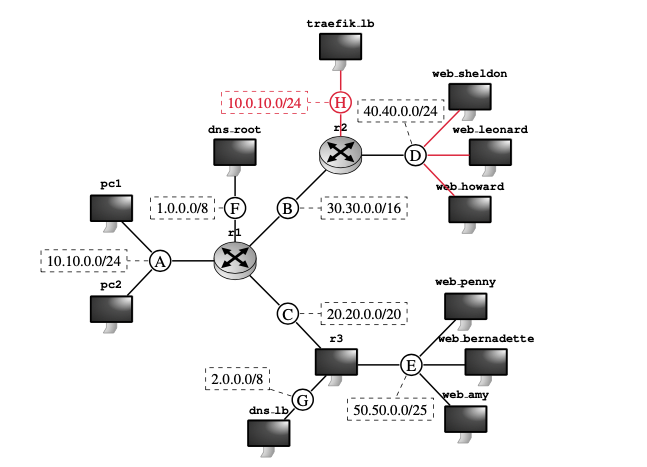
\includegraphics[width=0.9\textwidth]{Images/Replacing web1 with three new webservers..png}
  \caption{Experiment configuration with traefik}
  \label{fig:3.1}
\end{figure}
\subsection{Startup files}
Below mentioned are the start-up files of the new web servers.

\begin{figure}[H]
\centering
  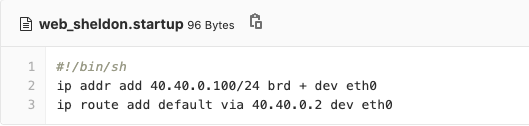
\includegraphics[width=0.9\textwidth]{Images/web_sheldon startup.png}
  \caption{web\textunderscore Sheldon startup}
  \label{fig:3.2}
\end{figure}

\begin{figure}[H]
\centering
  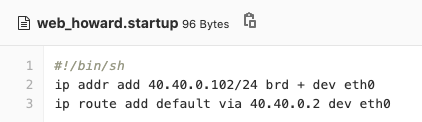
\includegraphics[width=0.9\textwidth]{Images/web_howard startup.png}
  \caption{web\textunderscore Howard startup}
  \label{fig:3.3}
\end{figure}

\begin{figure}[H]
\centering
  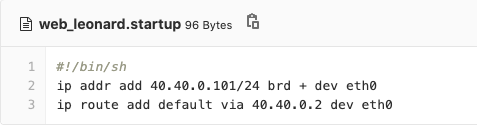
\includegraphics[width=0.9\textwidth]{Images/web_lenard startup.png}
  \caption{web\textunderscore Leonard startup}
  \label{fig:3.4}
\end{figure}

\begin{figure}[H]
\centering
  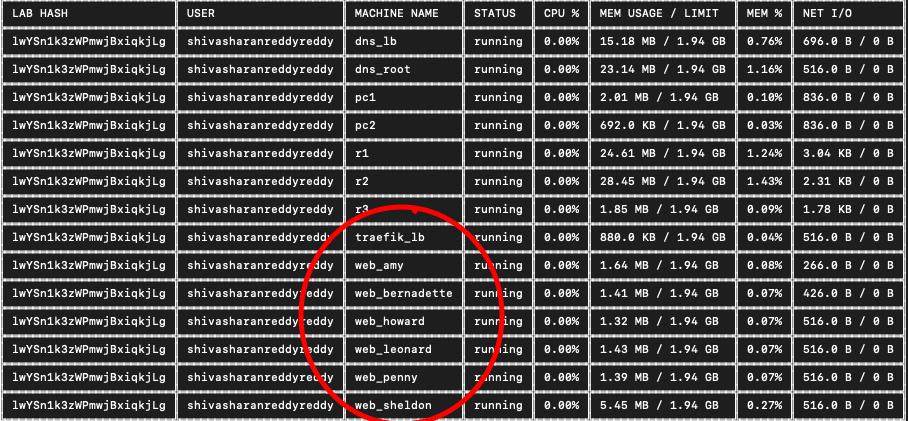
\includegraphics[width=0.9\textwidth]{Images/Web-1 Replaced .png}
  \caption{web\textunderscore 1 Replaced}
  \label{fig:3.5}
\end{figure}


\subsection{Connecting devices in the network}
We configure all three web servers in the network and try to reach them.

\begin{figure}[H]
\centering
  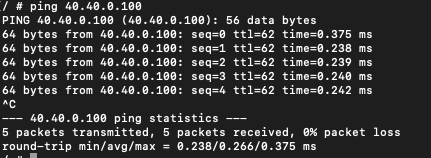
\includegraphics[width=0.9\textwidth]{Images/Connecting web-sheldon.png}
  \caption{Connecting web\textunderscore Sheldon}
  \label{fig:3.6}
\end{figure}

\begin{figure}[H]
\centering
  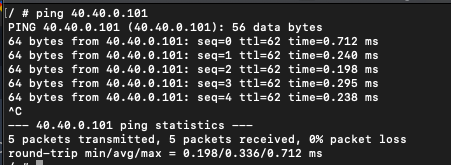
\includegraphics[width=0.9\textwidth]{Images/connecting web-howard.png}
  \caption{connecting web\textunderscore Howard}
  \label{fig:3.7}
\end{figure}

\begin{figure}[H]
\centering
  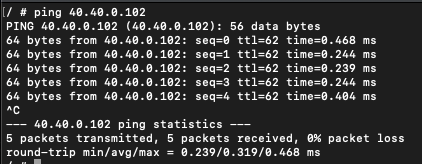
\includegraphics[width=0.9\textwidth]{Images/connecting web-lenard .png}
  \caption{connecting web\textunderscore Leonard}
  \label{fig:3.8}
\end{figure}



\section{Adding load-balancer traefik\textunderscore lb }
In this part we add loadbalancer traefik\textunderscore lb and configure it.

\begin{figure}[H]
\centering
  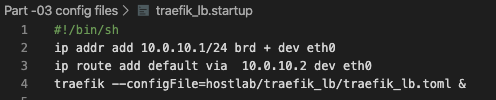
\includegraphics[width=0.9\textwidth]{Images/Traefik-lb start up.png}
  \caption{creating Traefik\textunderscore lb}
  \label{fig:3.9}
\end{figure}

\subsection{listen on port 80 and use a file provider}
This can be achieved by 'address' option at entry points.

\begin{figure}[H]
\centering
  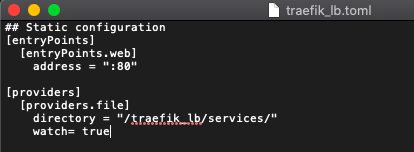
\includegraphics[width=0.9\textwidth]{Images/listen on port 80 and use a file provider,.png}
  \caption{Port 80}
  \label{fig:3.10}
\end{figure}

\subsection{which forwards requests on gik.de to the new web servers}

\begin{figure}[H]
\centering
  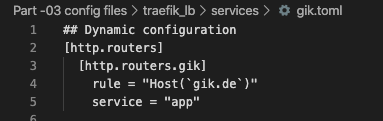
\includegraphics[width=0.9\textwidth]{Images/Request forwording.png}
  \caption{Request forwarding}
  \label{fig:3.11}
\end{figure}

\section{Adjusting the record of gik.de from dns root to point to traefik lb.}

\begin{figure}[H]
\centering
  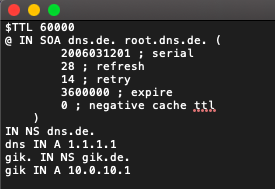
\includegraphics[width=0.9\textwidth]{Images/Adjusting a recored 3.3.png}
  \caption{Adjusting the record of gik.de from dns root to point to traefik\textunderscore lb}
  \label{fig:3.12}
\end{figure}

\section{Adding the static routes to the topology}
In this section we created three new web servers and a traefik\textunderscore lb so we are adding routing typologies for the same.

\subsection{web\textunderscore Sheldon routes}
\begin{figure}[H]
\centering
  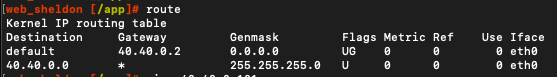
\includegraphics[width=0.9\textwidth]{Images/Web-sheldon routes.png}
  \caption{Web-Sheldon routes}
  \label{fig:3.13}
\end{figure}

\subsection{web\textunderscore Howard routes}
\begin{figure}[H]
\centering
  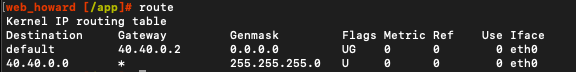
\includegraphics[width=0.9\textwidth]{Images/web-howard routes.png}
  \caption{Web-Howard routes}
  \label{fig:3.14}
\end{figure}

\subsection{web\textunderscore Leonard routes}
\begin{figure}[H]
\centering
  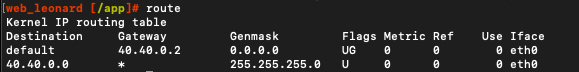
\includegraphics[width=0.9\textwidth]{Images/Web-leonard routes.png}
  \caption{Web\textunderscore Leonard routes}
  \label{fig:3.15}
\end{figure}

\subsection{Traefik\textunderscore lb routes}
\begin{figure}[H]
\centering
  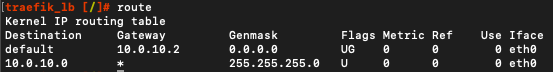
\includegraphics[width=0.9\textwidth]{Images/Traefik-lb route .png}
  \caption{Traefik\textunderscore lb routes}
  \label{fig:3.16}
\end{figure}

\section{Testing the load balancing behavior and add a weighted round robin to forward
}
 60 \% of the requests to web Sheldon,
 \\30 \% of the requests to web Leonard,
 \\and 10 \%  of the requests to web Howard.

\begin{figure}[H]
\centering
  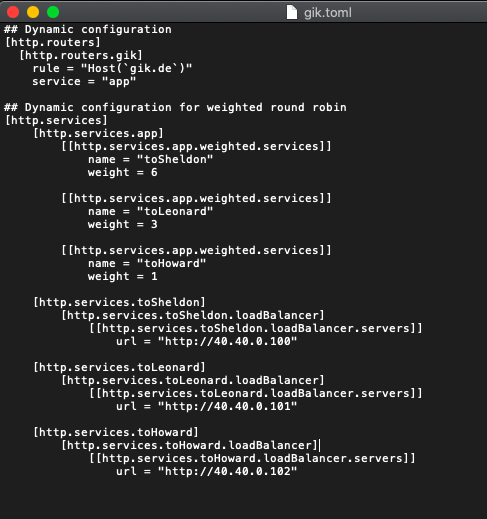
\includegraphics[width=0.9\textwidth]{Images/Round-Robin.png}
  \caption{Round robin}
  \label{fig:3.17}
\end{figure}

\section{Differences between DNS and software load balancing}
\begin{itemize}
\item Dns load balancing is easy to configure when compared to software load balancing 
\item In DNS we can assign multiple IP address but in software based load balancing it requires one specified ip address.
\item In DNS load balancing client request is forwarded to same server destination even if is overloaded, But in software based load balancing we dont observe this pit fall.

\subsection{pros and cons of DNS}

\item Easy to configure and understand.
\item Multiple IP addresses can be assigned to the host   record.It divides workload equally.
\item DNS based cluster nodes don’t require multiple network interface cards

\item No capability other than round-robin.
\item DNS cannot identify if the server is down.
\item Each server requires a different IP address

\subsection{Pros and cons of software load balancing}

\item Cost effective- we don't require physical hardware systems to perform the task.
\item It does not require a separate public IP for each server 

\item Compared to hardware load balancer, the main drawback to software load balancer is in its performance.

\end{itemize}
